%----------------------------------------------------------------------------------------
% Analytical Process
%----------------------------------------------------------------------------------------
\section{Analytical Process}\label{sec:analytical_process}

\subsection{Methodology}\label{sec:methodology}

\subsubsection{WiFi Provisioning through Bluetooth}

Internet of Things has brought about a need for efficient communication protocols for various devices, including the ESP32 microcontroller. The WiFi provisioning through Bluetooth is a novel method that enables streamlined configuration of the WiFi credentials of an ESP32 module through the use of a Bluetooth Low Energy (BLE)-enabled device, such as a smartphone.

The WiFi provisioning through Bluetooth consists of the following steps:

\begin{enumerate}
  \item The ESP32 module starts a BLE server with a predefined service UUID and advertises itself as a WiFi provisioning device.
  \item A BLE-enabled device scans for nearby BLE devices and connects to the ESP32 module using its service UUID, enabling communication between the devices.
  \item The BLE-enabled device sends a protobuf message to the ESP32 module using the \texttt{wifi\_scan endpoint}, requesting a list of available WiFi networks.
  \item The ESP32 module scans for nearby WiFi networks and sends back a protobuf message with the list of SSIDs and RSSIs to the BLE-enabled device using the \texttt{wifi\_scan} endpoint.
  \item The BLE-enabled device selects a WiFi network from the list and sends its SSID and password to the ESP32 module using the \texttt{wifi\_config} endpoint.
  \item The ESP32 module validates the credentials and attempts to connect to the selected WiFi network, sending back a protobuf message with the connection status (success or failure) to the BLE-enabled device using the \texttt{wifi\_config} endpoint. If the connection is successful, the ESP32 module obtains an Internet Protocol (IP) address from the WiFi network and stops advertising itself as a WiFi provisioning device. It also stops accepting any further provisioning requests from other devices. In the event of a connection failure, the ESP32 module resets its internal state machine and clears its provisioned credentials. It continues advertising itself as a WiFi provisioning device until it receives valid credentials or until it is manually stopped by calling the \texttt{wifi\_prov\_mgr\_stop\_provisioning()} function~\cite{espressif:esp-idf-programming-guide}.
\end{enumerate}

The WiFi provisioning through Bluetooth requires an application on both sides: one on the ESP32 module and one on the BLE-enabled device. Espressif provides an Android app that serves as a client~\cite{google-play:esp-ble-provisioning}.

Overall, the WiFi provisioning through Bluetooth method provides a solution for efficent WiFi configuration on ESP32 modules. This approach mitigates the need for hard-coded credentials or user input, simplifying the process for users to connect their devices to a WiFi network. Through the use of BLE-enabled devices, this method offers efficient and secure communication between devices, making it a potential solution in the realm of IoT.

\subsubsection{OTA Updates}

OTA (Over-The-Air) updates allow for remote firmware updates of the ESP32 board via a Wi-Fi connection, eliminating the need for a physical connection. This functionality is useful for devices deployed in remote or hard-to-reach locations.

To enable OTA updates on the ESP32, the partition table of the device must be configured with at least two "OTA app slot" partitions (i.e. \texttt{ota\_0} and \texttt{ota\_1}) and an "OTA Data Partition". 

We created an \texttt{energy\_gateway\_ota} esp-idf component that handles the initialization, download, verification, and activation of new firmware images from a given URL \cite{energy-gateway:github}. We used this component in our \texttt{main.c} file to check for updates periodically and perform them if available.

% TODO: Make figure reference better
The firmware image was hosted on a web server \ref{fig:web_server}. The web server was configured to serve the firmware image over HTTPS. The URL of the firmware image was then passed to the \texttt{energy\_gateway\_ota} component, which downloaded the image and verified its integrity. The component then activated the new firmware image by setting the boot partition to the OTA app slot that was not previously selected for booting. The component then rebooted the device, which would then boot into the new firmware image.

\begin{figure}[ht]
  \centering
  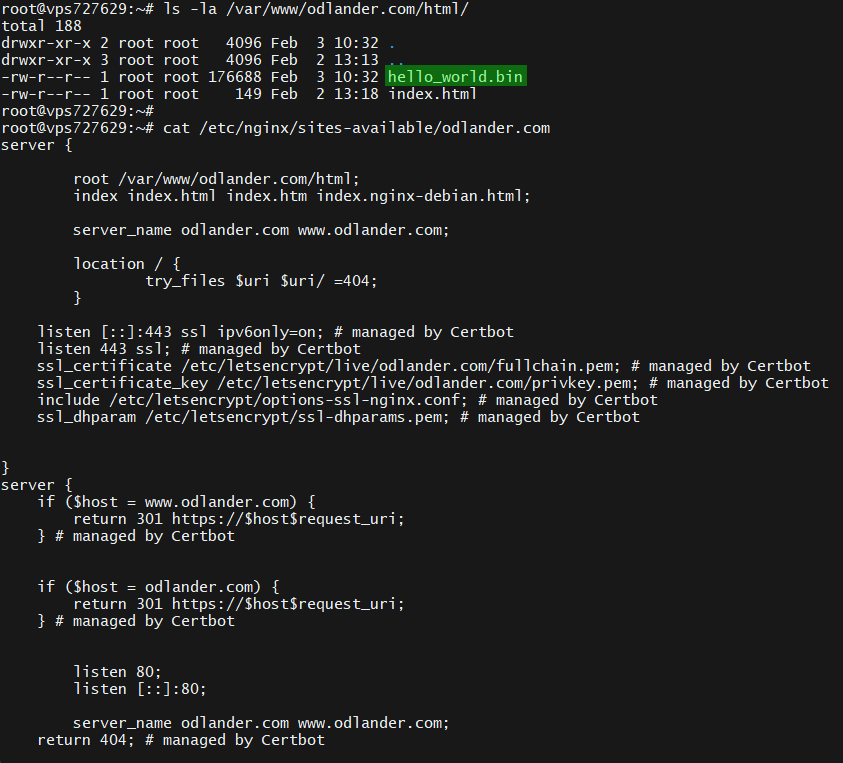
\includegraphics[width=0.8\linewidth]{figures/web_server.png}
  \caption{Web server}
  \label{fig:web_server}
\end{figure}

This also enables the possiblity for rollback to a previous firmware image in the event of a failed update \cite{espressif:esp-idf-programming-guide}. The \texttt{energy\_gateway\_ota} component stores the current firmware image version in the \texttt{ota\_data} partition. If the new firmware image fails to boot, the component could automatically rollback to the previous firmware image. This rollback functionality was not implemented in our project.

\subsubsection{UART communication}

\begin{figure}[ht]
  \centering
  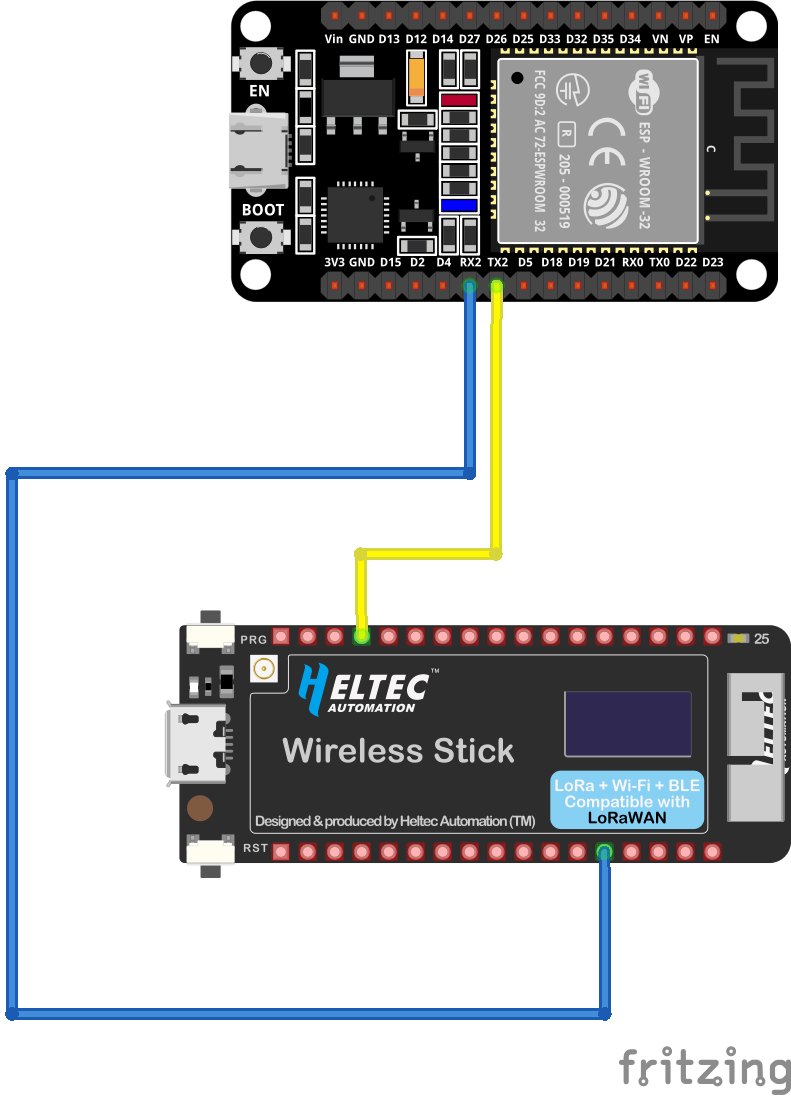
\includegraphics[width=0.8\linewidth]{figures/uart_connection.png}
  \caption{UART connection scheme}
  \label{fig:uart_connection}
\end{figure}

The Energy Gateway's final product requires the capability to poll from and send data to serial devices. To fulfill this requirement, we utilized the UART (Universal Asynchronous Receiver/Transmitter) protocol, which enables asynchronous communication between two devices in a full-duplex manner. The UART protocol is widely utilized in embedded systems, like the ESP32, to interface with sensors and actuators.

To simulate the UART protocol, we established a Heltec Wireless Stick as a serial device and connected it to the ESP32 module via UART (refer to Figure \ref{fig:uart_connection}). We programmed the ESP32 module to request data from the Heltec Wireless Stick at a rate of 20Hz, while the Heltec Wireless Stick was programmed to transmit a random number between 0 and 255 to the ESP32 module every 50ms. The ESP32 module then evaluated whether the received data was too high or low. If the data was deemed too low, a 0 was dispatched to the Heltec Wireless Stick, and if it was too high, a 1 was transmitted. Our solution passed our testing and in the final Energy Gateway product, the ESP32 module will acquire data from the serial device only at a rate of 2Hz.

\subsection{Concurrency}

When it comes to developing software with the Espressif IoT Development Framework (ESP-IDF), understanding the intricacies of priority levels is paramount for effective task management~\cite{Davis:2016}. The underlying operating system for ESP-IDF is FreeRTOS, which is a real-time operating system designed for microcontrollers that provides a multitasking environment for running multiple tasks simultaneously on a single processor. The priority-based preemptive scheduling algorithm employed by FreeRTOS is an essential feature that allows for efficient task management~\cite{espressif:esp-idf-programming-guide}.

ESP-IDF utilizes a range of 26 priority levels, numbered from 0 (highest) to 25 (lowest). The variable \texttt{ESP\_TASK\_PRIO\_MAX}, which represents the maximum allowed priority level in ESP-IDF, is currently set to 25 and can be found in the FreeRTOSConfig.h file\cite{espressif:freertosconfig}. This limitation ensures that the system remains stable and responsive, even when multiple high-priority tasks are running concurrently. By utilizing these priority levels effectively, developers can optimize system performance and ensure that critical tasks receive the necessary resources to execute efficiently~\cite{espressif:esp-idf-programming-guide}.

Choosing the appropriate priority level for a task requires careful consideration of its criticality and potential impact on the system. For instance, a high-priority task that reads data from a serial port demands immediate attention to avoid data loss or errors. In our project, we assigned a priority level of \texttt{ESP\_TASK\_PRIO\_MAX - 6} (level 19) to our serial-reading task. This priority level strikes a balance between prioritizing our task and allowing other tasks to run when needed. It also provides some headroom above the default priority levels of many other tasks in the system~\cite{espressif:esp-idf-programming-guide}, ensuring that our task receives immediate attention while still allowing for efficient resource allocation.

Moreover, it is worth noting that prioritization is not a one-size-fits-all solution. Different tasks have different criticality levels, and thus require different priority levels. Some tasks may be less critical but more time-consuming, while others may require frequent access to system resources. As such, the priority level should be carefully selected to ensure efficient task management and optimize system performance.

In conclusion, understanding the intricacies of priority levels is essential when programming with esp-idf. By choosing the appropriate priority level for each task, we can ensure efficient task management, avoid system performance degradation, and optimize system performance. With only 25 priority levels in ESP-IDF, developers have limited flexibility to assign priority levels based on the specific needs of their projects.

\subsection{Result}\label{sec:result}

\subsubsection{WiFi Provisioning through Bluetooth}

The WiFi provisioning through Bluetooth system was successfully developed and implemented on the ESP32 microcontroller. The system enables efficient configuration of WiFi credentials on ESP32 devices through the use of a BLE-enabled device. The system was tested, and it was found to be reliable and effective in provisioning WiFi credentials without the need for code modification. The system was integrated as a component using the ESP-IDF framework, enabling easy integration by other developers. The use of BLE-enabled devices enhances security, making it a potential solution in the realm of IoT.

\subsubsection{OTA Updates}

The OTA update system was successfully developed and implemented on the ESP32 microcontroller. The system allows for remote firmware updates of the ESP32 board via a Wi-Fi connection, eliminating the need for a physical connection. The system was tested, and it was found to be reliable and effective in updating the firmware image without interrupting any critical tasks that the unit may be currently running. The \texttt{energy\_gateway\_ota} component was utilized to handle the initialization, download, verification, and activation of new firmware images. The component also integrates git tags as a versioning system, resulting in the update being aborted if the tags differ. The system also enables the possibility for rollback to a previous firmware image in the event of a failed update. However, this rollback functionality was not implemented in our project.

\subsubsection{UART Communication}

The implementation of serial communication on the ESP32 microcontroller was successful. The microcontroller was connected to a Heltec Wireless Stick~\ref{fig:serial_connection} and able to establish a serial communication channel with the Stick, running MicroPython, to receive and transmit data. The Wireless Stick was programmed to send random integers between 0 and 255 over serial at an interval. The ESP32 used the \texttt{uart\_read\_bytes(ECHO\_UART\_PORT\_NUM, (char *) uartData, (UART\_BUF\_SIZE - 1), 20 / portTICK\_PERIOD\_MS);} function call, to read the bytes, with a timeout of 20 milliseconds, and place them in the \texttt{uartData} buffer. When a value greater than 250 or less than 5 was received, the microcontroller send back a value of 1 or 0, respectively, to the Wireless Stick. After every transmission, the buffer was cleared and the task yielded for 10 milliseconds, using \texttt{vTaskDelay(10 / portTICK\_PERIOD\_MS);} to not starve other tasks of resources.

The sending interval was tested at different frequencies, with promising results. When no other tasks were running, the device managed to catch all values sent at a data rate of 33Hz. Enabling the OTA task and running it every five seconds, the device was able to catch all values sent when the data rate was reduced to 20Hz.

\begin{figure}[ht]
  \centering
  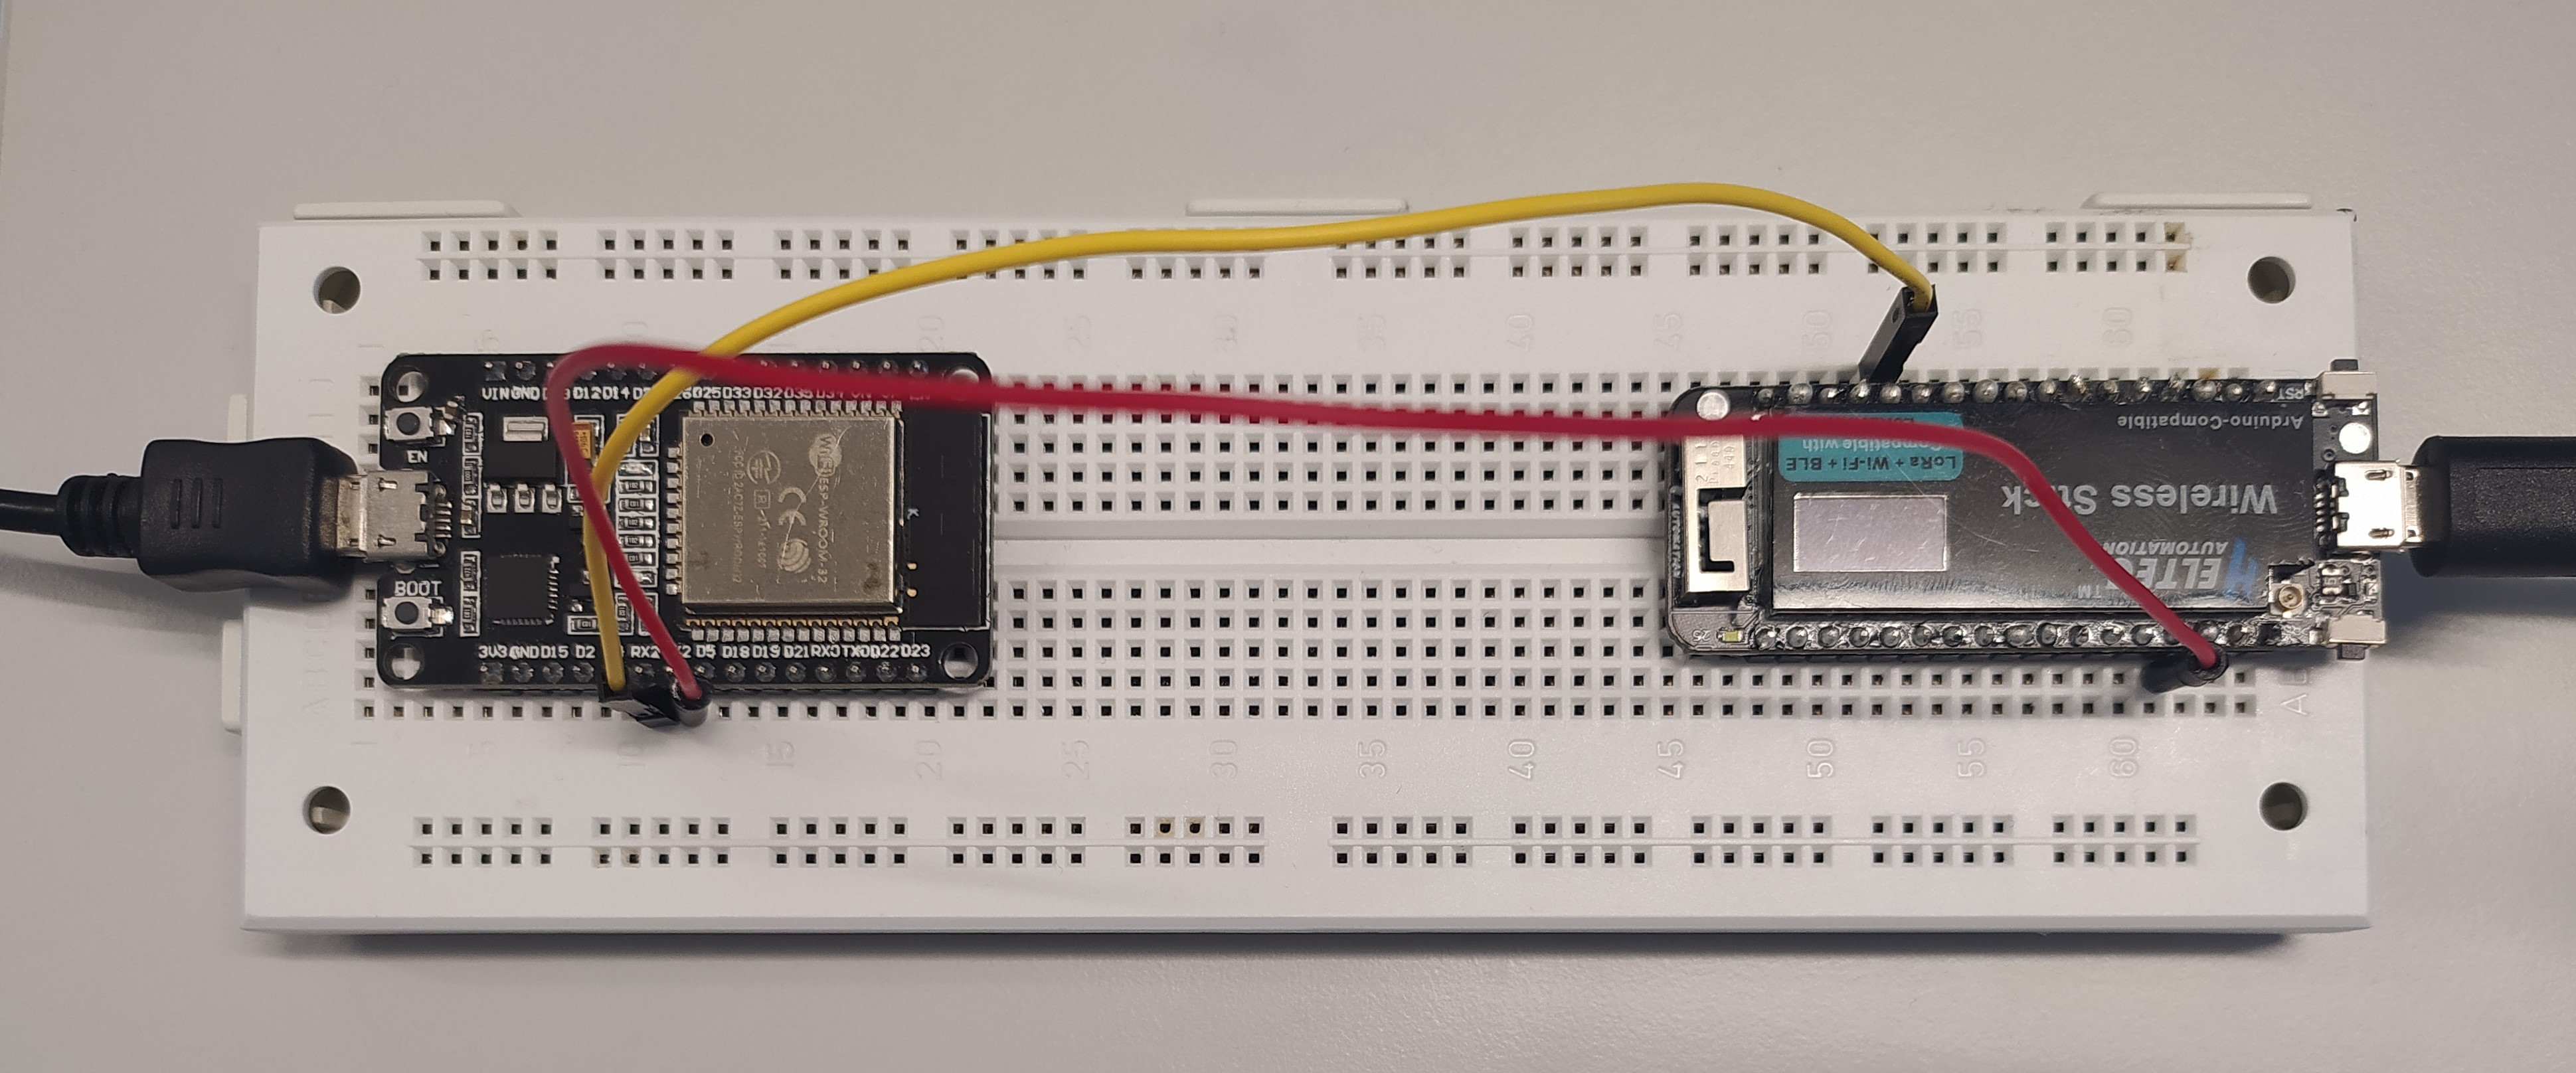
\includegraphics[width=0.8\linewidth]{figures/serial_connection.jpg}
  \caption{ESP32 connected via serial}
  \label{fig:serial_connection}
\end{figure}

\begin{figure}[ht]
  \centering
  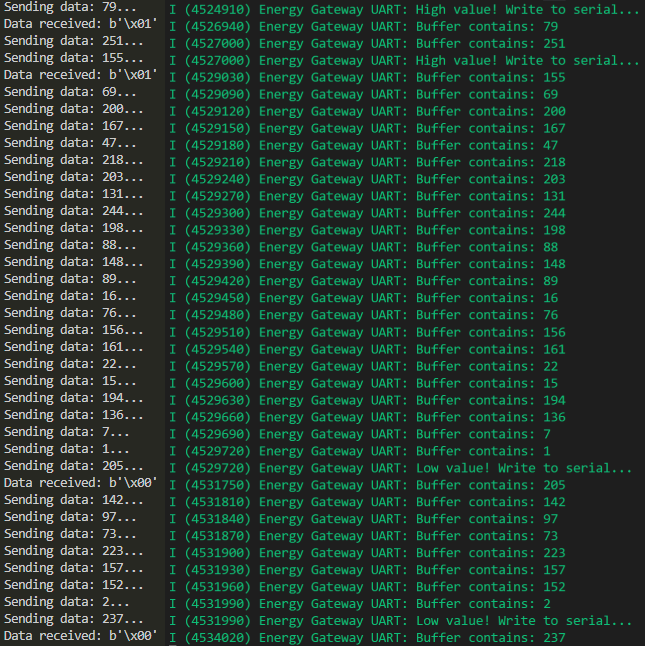
\includegraphics[width=0.8\linewidth]{figures/send_receive_33Hz.png}
  \caption{Serial communication at 33Hz}
  \label{fig:serial_communication_33hz}
\end{figure}

\subsubsection{Concurrency}

\begin{table}[ht]
  \centering
  \caption{Task priority levels}
  \label{table:task-priorities}
  \begin{tabularx}{\textwidth}{p{1cm}Xp{10cm}}
    \hline
    \textbf{Priority} & \textbf{Example task} & \textbf{Description} \\ 
    \hline
    0 & \texttt{IDLE} & Idle tasks. \\
    \hline
    1 & \texttt{app\_main} & These are the tasks we prioritize the least.\\
    \hline
    2 & \texttt{ota\_task} & Tasks in this priority are prioritized very low.\\
    \hline
    18 & \texttt{tcpip\_task} & Important border. Tasks with higher priority than this can not be guaranteed to perform network operations as its possible they will override the TCP/IP stack. \\
    \hline
    19 & \texttt{uart\_task} & Using priority 19 or higher will guarantee an application task can run on Core 1 without being preempted by any built-in task\cite{espressif:esp-idf-programming-guide}. \\
    \hline
    20 & \texttt{event\_task} & The event handling system task to manage the default system event loop and execute callbacks. \\
    \hline
    22 & \texttt{esptimer\_task} & High Resolution Timer (ESP Timer) system task to manage high precision timer events and execute callbacks. \\
    \hline
    25 & \texttt{none} & Max Priority \\
    \hline
  \end{tabularx}
\end{table}

First task thats creates is the UART task, which is given a priority of 19. This task is responsible for receiving data from the Wireless Stick and sending data back to the Wireless Stick. The task is given a priority of 19 to ensure that it is not preempted by any other tasks. The task is then put into a while loop, where it waits for data to be received. When data is received, the task checks if the data is greater than 250 or less than 5. If the data is greater than 250, the task sends a value of 1 back to the Wireless Stick. If the data is less than 5, the task sends a value of 0 back to the Wireless Stick. The task then yields for 10 milliseconds, using \texttt{vTaskDelay(10 / portTICK\_PERIOD\_MS);}.

After the UART task is created, the OTA task is created. This task is given a priority of 2. This task is responsible for checking for new firmware images and updating the firmware image if a new one is available. The task is given a priority of 2 to ensure that it does not preemp any other tasks. After the task has been run once its removed from the task list, a timer is started that will run the task again after 24 hours. When the timer expires, the task is once again placed in the task list, on a low priority of 2.
